\begin{XeClass}{FsUrlStreamHandlerFactory}
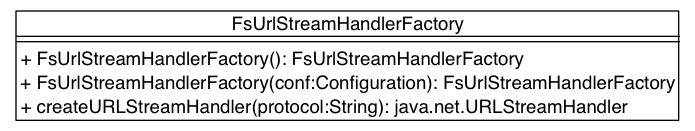
\includegraphics[width=10cm]{cdig/FsUrlStreamHandlerFactory.png}
     
 FsUrlStreamHandlerFactory是由多个URL流输入输出处理器组成的工厂方法,
 实现了URLStreamHandlerFactory接口,
 拥有三个私有的成员变量: Configuration对象conf,
 HashMap<String, Boolean>对象 protocols,
 还有private java.net.URLStreamHandler对象handler.
 在众多的类中只有一个处理器的工作是生成UrlConnections对象,
 UrlConnections类依赖于FileSystem并选择合适的接口进行实现.
 在createURLStreamHandler方法中返回handler之前,
 需要FileSystem类的实现接口中明确清楚传入需要的参数

    \begin{XeMethod}{\XePublic}{FsUrlStreamHandlerFactory}{FsUrlStreamHandlerFactory}
         
 FsUrlStreamHandlerFactory第一个构造函数
 conf引用到一个新创建的Configuration类对象中
 确定了conf的值后调用FsUrlStreamHandler
 并将返回值赋值给handler

    \end{XeMethod}

    \begin{XeMethod}{\XePublic}{FsUrlStreamHandlerFactory}{FsUrlStreamHandlerFactory}
         
 FsUrlStreamHandlerFactory第二个构造函数
 conf引用到一个配置好的Configuration类对象中
 确定了conf的值后调用FsUrlStreamHandler
 并将返回值赋值给handler

    \end{XeMethod}

    \begin{XeMethod}{\XePublic}{java.net.URLStreamHandler}{createURLStreamHandler}
         
 FsUrlStreamHandlerFactory第二个构造函数
 createURLStreamHandler接收一个String参数protocol
 判断protocols字典中是否存在这个protocol
 若存在则将handler变量返回,不然则返回null

    \end{XeMethod}

\end{XeClass}
